
\begin{abstract}
There is limited evidence on the labour market impact of diabetes, and existing evidence tends to be weakly identified. Making use of Mexican panel data to estimate individual fixed effects models, we find evidence for adverse effects of self-reported diabetes on employment probabilities, but not on wages or hours worked. Complementary biomarker information for a cross section indicates that a large diabetes population is unaware of the disease. When accounting for this, the negative relationship of self-reported diabetes with employment remains, but does not extend to those unaware of their diabetes. Further analysis suggests that this difference stems from worse general health among the self-reports rather than more severe diabetes.
\end{abstract}



\section{\label{sec:Introduction4}Introduction }

Diabetes, and particularly its most common variant, type 2 diabetes, has increased worldwide and is expected to continue to rise over the next decades \parencite{Risk2016}. It has become a problem for \acp{MIC} and \acp{HIC} alike, with over two-thirds of people with diabetes living in the developing world \parencite{InternationalDiabetesFederation2013}. Mexicans and Mexican-Americans appear to be particularly affected by diabetes, also in comparison to other Latino populations living in the USA \parencite{Schneiderman2014}. In Mexico itself, diabetes prevalence has been estimated to have grown from 6.7\% in 1994 to 14.4\% in 2006, including both diagnosed and undiagnosed cases \parencite{Barquera2013}, and is expected to increase further over the next decades \parencite{Meza2015}. Already now, diabetes is the number one cause of death in Mexico \parencite{Barquera2013}. 

The observed trend has been attributed to a deterioration in diet and a reduction in physical activity \parencite{Barquera2008b,Basu2013}, while genetic predisposition among Mexicans with pre-hispanic ancestry may also have played a role \parencite{Williams2013}. Recent evidence indicates that the onset of diabetes has been occurring at an ever earlier age in Mexico \parencite{Villalpando2010}. With treatment as ineffective as it currently is---only a minority achieves adequate blood glucose control \parencite{Barquera2013}---the earlier onset will increase the likelihood of complications during the productive lifespan. 

Diabetes is a term used to describe various conditions characterized by high blood glucose values, with the predominant disease being type 2 diabetes accounting for about 90 \%of all diabetes cases \parencite{Sicree2009}. The elevated
blood glucose levels that are a result of the body's inability to use insulin properly to maintain blood glucose at normal levels, can entail a range of adverse health effects for the individual concerned. However, via effective self-management of the disease much if not all of the complications can be avoided \parencite{Lim2011, Gregg2012}. In the absence of effective self-management---or in the case of inadequate treatment---diabetes has been documented to lead to conditions such as heart disease and stroke, blindness, kidney problems, and nerve problems which together with impaired wound healing can lead to the loss of limbs \parencite{Reynoso-Noveron2011}. These conditions can be seriously debilitating and may therefore reduce an individual's economic activity, including its productivity and labour market participation.

The effect of diabetes on labour market outcomes has been studied predominantly in \acp{HIC}---with the exception of a study on Mexico \autocite{Seuring2015} and one on China \parencite{Liu2014} each. In the \ac{HIC} studies diabetes has been found to be associated with reductions in employment probabilities as well as wages and labour supply \parencite{Brown2005,Brown2014,BrownIII2011,Minor2011,Minor2013,Minor2015,Latif2009,Seuring2015a}.

While these studies have provided useful evidence on the potential labour market effects of diabetes, many of the complexities of the relationship have not been comprehensively addressed in any given study. First of all, unobserved heterogeneity presents a challenge to estimate the relationship between diabetes and labour outcomes. Especially time-invariant unobserved individual characteristics, e.g. health endowments---often related to health during uteru, infant and child years, and to low household income or adverse health shocks during these early years---as well as risk preferences have been shown to adversely affect health in general and the propensity to develop type 2 diabetes more specifically \parencite{VanEwijk2011,Sotomayor2013,Li2010b}. These and other unobserved personal characteristics (e.g. ability) may also affect employment probabilities, wages or working hours directly through their effects on contemporaneous productivity \parencite{Currie2013} and indirectly by limiting educational attainment and human capital accumulation \parencite{Ayyagari2011a}. Further, only focusing on the overall effect of a self-reported diabetes diagnosis does not reveal when potential labour market penalties appear, given the dynamic aspect of diabetes and the potential differences in its effects over time. Additionally, apart from its health impact diabetes might also affect labour market outcomes through other channels. For instance, people aware of their condition may be less inclined to continue working if this interferes with their disease management or be suffering from psychological consequences (depression, anxiety) of becoming aware of the disease; they may also use the diagnosis as a justification for decreasing their labour supply, leading to a potential justification bias in the estimated effect of diabetes \parencite{Kapteyn2009}. Importantly, for these reasons the labour market effects may also be distinct for people with self-reported versus those unaware of their condition, potentially leading to biased estimates if the analysis is solely based on self-reports.

The objective of this study is to provide new evidence on the impact of diabetes on labour outcomes, while improving upon previous work by paying close attention to the above challenges. We use three waves of panel data from Mexico covering the period 2002--2012, provided by the \ac{MxFLS}. The \ac{MxFLS} is particularly useful for the analysis of diabetes as it allows us to account for the above complexities in a more refined way than has been the case so far. Using individual level \ac{FE} analysis for the first time in this literature, we take account of time-invariant heterogeneity when assessing the impact of self-reported diabetes and self-reported diabetes duration on labour market outcomes.\footnote{We are not aware of any other evidence on the effect on wages and working hours in a \ac{MIC}.} Further, we add to the current literature in exploring the role of undiagnosed diabetes, using novel and rich biomarker data---an issue of considerable importance in light of the large prevalence of undiagnosed diabetes (see \textcite{Beagley2014}) that remained unaccounted for in most earlier studies which typically rely on self-reported information. Doing so sheds light on the issue of measurement error and the potentially differential effects of self-reported and undiagnosed diabetes. 

Our results using self-reported diabetes suggest an economically important decrease in the employment probability of people aware of their disease. Wages and working hours, however, do not appear to be negatively associated with self-reported diabetes. We further find that employment probabilities are reduced with each additional year since diagnosis, with some evidence for an even larger effect per year after the initial 10 years. 

The biomarker analysis indicates that self-reported diabetes entails a significant employment penalty, while biometrically measured diabetes does not. Overall, undiagnosed diabetes does not appear to affect any of the labour market outcomes examined here, suggesting that adverse effects mainly occur to those self-reporting a diagnosis. We argue that, nonetheless, the effects found for self-reported diabetes in this study are largely unbiased as long as inference is not extended to the unobserved undiagnosed population, and are economically important in light of the sheer size of the diagnosed population in Mexico.


\section{\label{sec:Labor  outcomes and diabetes literature}Diabetes and labour outcomes---existing evidence}

Several studies have investigated the effects of diabetes on labour market outcomes. 

For the USA, \textcite{Brown2005} estimate  the impact on employment in 1996--1997 in an elderly population of Mexican Americans living close to the Mexican border, using a bivariate probit model. The study finds diabetes to be endogenous for women but not for men.  For the latter, the estimates show a significant adverse effect of 7 percentage points. For women, the negative effect becomes insignificant when using \ac{IV} estimation. In another study, again for a cross-sectional sample of  Mexican-Americans, \textcite{BrownIII2011} look at how diabetes management, inferred from measured \ac{HbA1c} levels, is associated with employment chances and wages. The authors detect a linear negative association between \ac{HbA1c} levels and both employment chances and wages for men. 

Two further studies also examine the impact of diabetes on employment and productivity for the USA: \textcite{Minor2011} focuses on the effect of diabetes on female employment, earnings, working hours and lost work days in 2006, finding diabetes to be endogenous and its effect underestimated if exogeneity is assumed. In the \ac{IV} estimates, diabetes has a significant negative effect on female employment as well as annual earnings but not on working hours. In a later study \textcite{Minor2013} investigates the relationship of diabetes duration and labour market outcomes using a cross-sectional analysis, providing evidence of a non-linear relationship, with employment probabilities declining shortly after diagnosis for men and after about 10 years for women; wages are not affected by duration. Finally, a recent study by \textcite{Minor2015} investigates the association of self-reported diabetes and undiagnosed diabetes with employment probabilities and working hours in an adult USA population, using cross-sectional data. This study indicates a reduction in the coefficient size of diabetes if undiagnosed diabetes cases are included in the diabetes indicator instead of only self-reported diabetes. Further, they find that there is no association of undiagnosed diabetes with employment probabilities itself. However, the results of the study, particularly those for undiagnosed diabetes, are based on a very small number of cases, warranting further investigation.

For Canada, \textcite{Latif2009} estimate the effect of the disease on employment probabilities using an \ac{IV} strategy similar to \textcite{Brown2005}. His results suggest diabetes to be exogenous for females, and both endogenous and overestimated for males in the univariate model, with the estimates of the bivariate model indicating a significant negative impact on the employment probabilities for women, but not for men. For Australia, \textcite{Zhang2009} analyse the effects of diabetes on labour force participation using a multivariate endogenous probit model. Their results demonstrate reduced labour market participation for males and females as a result of diabetes, with the effects appearing overstated if the endogeneity of diabetes is unaccounted for. 

To the best of our knowledge only two studies exist for non-\acp{HIC}. \textcite{Liu2014} investigate the effect of a diabetes diagnosis on labour income in China, exploiting a natural experiment to identify causality and find a significant reduction in income for those with a recent diagnosis. An earlier study for Mexico explored the effect of self-reported diabetes on the probability of employment using only cross-sectional data from the 2005 wave of the \ac{MxFLS}, and found a significant (p<0.01) reduction in employment chances for males by about 10 percentage points and for females by about 4.5  percentage points (p<0.1), using parental diabetes as an \ac{IV} \parencite{Seuring2015}. The scarcity of evidence for \acp{LMIC} is also documented in a recent systematic review of the economic cost of diabetes \parencite{Seuring2015a}. 


Overall, the majority of existing studies, including those on high income countries, tend to suffer from at least four key limitations: 
\begin{enumerate}
\item  They rely exclusively on cross-sectional data, limiting the possibilities to account for unobserved individual characteristics.
\item The use of the family history of diabetes, which has been the sole instrumental variable employed so far, relies on the genetic and heritable component of type 2 diabetes that could theoretically provide valid identification of the true effect of diabetes. However, it remains unclear whether the variable fully satisfies the exclusion restriction, as it may also proxy for other genetically transferred traits, including unobserved abilities that impact labour outcomes directly. This traditional identification strategy also abstracts from intrahousehold or intergenerational labour supply effects \parencite{Seuring2015}.\footnote{It is conceivable that diabetes might deteriorate parental health in such a way that the offspring either has to give up their employment to provide care, or has to increase labour supply to compensate for lost income.}
\item The use of self-reported diabetes can introduce non-classical measurement error due to systematic misreporting which has been shown to cause estimates of economic impacts to be potentially biased and overstated \parencite{Cawley2015,ONeill2013,Perks2015}.
\item A final potential limitation lies in the selection into diagnosis as a result of disease severity: those who are more severely ill are more likely to have visited a medical doctor and be diagnosed.  
\end{enumerate}

To overcome some of these limitations, this paper applies an individual level \ac{FE} panel estimation strategy and makes use of biomarker data. We also estimate models for different types of employment, i.e. non-agricultural wage employment, agricultural employment and self-employment, as ill health may have distinct effects across these activities.
\section{\label{sec:Data}Data}

We use the \acf{MxFLS}, a nationally representative, longitudinal household survey, which has three waves conducted in 2002, 2005--2006 and 2009--2012. All household members aged 15 and above were interviewed, covering information on a wide range of social, demographic, economic and health characteristics of the individuals and their families \parencite{Rubalcava2013}. Apart from self-reported diabetes information that is available in all rounds, we also use information on the self-reported year of diagnosis as well as biomarker data including \ac{HbA1c} levels for a subsample of respondents.  Our main analysis uses all three waves taking advantage of the large amount of observations and the panel structure of the data. Our variable of interest is self-reported diabetes, which is based on the survey question: "Have you ever been diagnosed with diabetes?". 



Because the response to this question may well suffer from measurement error due to recall bias, we investigate and try to increase the consistency of the self-reported diabetes variable, using disease information from earlier and ensuing waves to infer on the current, missing or inconsistent, diabetes status. One of the key advantages of panel data is the repeated measurement giving more than one data point for many of the individuals, thereby allowing to uncover inconsistencies for those with at least two observations. While we are not aware of any literature investigating the issue of inconsistencies in self-reported diabetes over time, a study by \textcite{Zajacova2010}, on the consistency of a self-reported cancer diagnosis over time in a USA population, found that 30\% of those who had reported a cancer diagnosis at an earlier point did report at a later point that they never had received a cancer diagnosis. They also found that a more recent diagnosis was reported with greater consistency possibly due to increasing recall problems and/or reduced salience as time since diagnosis progresses.

We also find inconsistencies in the diabetes self-reports over the three waves of the \ac{MxFLS} data, with between 10--20\% of those reporting diabetes in one wave not doing so in one of the subsequent waves. In order to reduce the amount of inconsistencies, we were interested in the validity of diabetes self-reports. While we could not find a study assessing the validity of self-reported diabetes in Mexico, a study from China has shown that specificity of self-reported diabetes, i.e. those who self-report a diabetes diagnosis actually have diabetes, was very high (>98\% for China), while sensitivity, i.e. how many people with diabetes, diagnosed or undiagnosed, actually self-report the disease, was low (40\% for China) \parencite{Yuan2015}. This indicates that people who report a diabetes diagnosis are likely to indeed have the condition while many of those not reporting a diabetes diagnosis are unaware of their diabetes.

We assess the validity of self-reported diabetes in our data by using \ac{HbA1c} levels and the self-reports of diabetes related medicine use from wave three. We find that 90\% of those self-reporting a diabetes diagnosis had an \ac{HbA1c} $\geq6.5$\% or did report taking diabetes medication, indicating relatively high specificity in our data as well.

We used this information to infer the "true" diabetes status for those with inconsistent reports. For those with two waves, we assumed that if a diabetes diagnosis had been reported in a prior wave they also had diabetes in the ensuing wave, even if then it was not reported.
For people where we had data from all three waves, we used that additional information to make a decision on how to deal with inconsistencies using the rules outlined in Table \ref{tab:Inconsistencies}

\begin{table}[h!]
\caption{\label{tab:Inconsistencies}Inconsistencies in diabetes self-report in MxFLS.}
\begin{center}
\begin{adjustbox}{max width=\linewidth} 
\begin{tabular}{llc}
\hline 
Inconsistency  & Assumption  & Number of observations replaced\tabularnewline
\hline 
Diabetes self report in 2002, 2005 but not in 2009  & Has diabetes in 2009 as well  & 19\tabularnewline
Diabetes self report in 2002, 2009 but not in 2005  & Has diabetes in 2005 as well  & 63\tabularnewline
Diabetes self report only in 2002, but not in 2005 and 2009  & Has no diabetes in 2002 either  & 66\tabularnewline
Diabetes self report only in 2005, but not in 2002 and 2009  & Has no diabetes in 2005 either  & 52\tabularnewline
Diabetes self report in 2002, but not in 2005. Not in survey in 2009  & Has diabetes in 2005 as well  & 44\tabularnewline
Diabetes self report in 2005, but not in 2009. Not in survey in 2002  & Has diabetes in 2009 as well  & 23\tabularnewline
\end{tabular}
\end{adjustbox}
\end{center}
\end{table}


This approach should add more consistency to the self-reported diabetes information by using all available information. We tested if this approach was supported by the \ac{HbA1c} values provided in wave 3. Of those with inconsistencies in their diabetes elf-reports 95 were present in the biomarker sample (46 with two and 49 with one self-report of diabetes). We therefore  Using a t-test we compared the mean \ac{HbA1c} for the two groups and found a significantly (p<0.001) higher mean \ac{HbA1c} (9.7\%) for those with two self-reports compared to for those with only one self-report of diabetes (7.0\%). Further, of those with one self-report, for only 30\% the \ac{HbA1c}$\geq6.5$\% compared to 87\% of those with two self-reports. Based on these results we are reassured that the way we have dealt with the inconsistencies in the data minimizes misclassification of people into diabetes or no-diabetes and has reduced some of the measurement error in the diabetes data. Unfortunately we cannot use a similar method for dealing with inconsistencies in the self-reported year of diabetes diagnosis, as it has only been reported once. Hence, the results from duration analysis should be interpreted with care.


 A further, and no less important, source of measurement error is the omission of those with undiagnosed diabetes. In order to investigate how this may affect estimates of the labour market impact of diabetes we use information from a subsample of the 2009-2012 wave containing over 6000 respondents (everybody aged 45+  and a random subsample of those aged 15--44 \parencite{Crimmins2015}) that have biometrically measured blood glucose values, allowing for the identification of those with undiagnosed diabetes. 
Throughout our analysis the samples we use are restricted to the working age population (15--64). To prevent pregnant women from biasing our results due to the increased diabetes risk during pregnancy and its effects on female employment status, we have dropped all observations of women reporting to be pregnant at the time of the survey (N=764). We further exclude everybody currently in school.

The detailed information in the \ac{MxFLS} allows us to consider the following outcome variables of interest: employment\footnote{Employment status is defined as having worked or carried out an activity that helped with the household expenses the last week and working for at least four hours per week. This explicitly includes those employed informally, for instance people working in a family business. The number of working hours needed to be considered as working is lower than in Chapter \ref{cha:Mex1}. We took this decision because we wanted to assess the impact of diabetes on driving people out of work completely. Any effect on working hours should be captured in the respective working hours models. We also tested if changing the definition of being employed to having worked at least ten hours per week as in Chapter \ref{cha:Mex1}. This only led to marginal changes in the coefficients and standard errors, not affecting the interpretation of the results.}, hourly wage and weekly working hours.\footnote{Hourly wage was calculated by adding up the reported monthly income from the first and second job (if any) and dividing it by the average number of weeks per month. This gave us the average earnings per week which were then divided by the weekly working hours to arrive at an hourly wage estimate. Labor income was either reported as the total amount for the whole month or more detailed containing information on the monthly wage, income from piecework, tips, extra hours, meals, housing, transport, medical benefits and other earnings. Over 80\% of respondents reported the total amount instead of a detailed amount. Respondents were also asked for their annual income and we used that information to arrive at an hourly wage if information for monthly labour income was missing. Finally, we adjusted the calculated wage for inflation from the year of the interview up to 2013 and took the log of those values. Due to a considerable number of missing or zero income reports the sample used for the wage estimation is smaller than the sample for working hours. Working hours were calculated summing up the self-reported working hours of the first and---if applicable---the second job.} For the pooled data of all three waves (Table  \ref{tab:Pooled-sample-characteristics}), diabetes was self-reported by 5\% of men and 6\% of women, respectively. This is consistent with other prevalence estimates of self-reported diabetes for this time period in Mexico.\footnote{\textcite{Barquera2013} show that the prevalence of diagnosed diabetes in Mexico was 7.5\% in 2006, only somewhat above our results, which may be the result of the slightly different age groups considered.}  About half of the respondents in the sample live in rural areas. Looking at our outcome variables, 86\% of men report some form of employment compared to 37\% of women. Interestingly, men do not report considerably higher hourly wages than women but work more hours per week. Also, men are working more often in agricultural jobs while women are more likely to be self-employed or in non-agricultural wage employment. Women also have lower educational attainment on average. 

\begin{table}
\caption{\label{tab:Pooled-sample-characteristics}Descriptive statistics for panel and biomarker sample.}

\begin{threeparttable}  %adds notes to tables

{
\def\sym#1{\ifmmode^{#1}\else\(^{#1}\)\fi}
\begin{adjustbox}{max width=1\linewidth, center}
\begin{tabular}{l*{4}{c}}
\toprule
                    &\multicolumn{2}{c}{Panel}&\multicolumn{2}{c}{Biomarker}\\\cmidrule(lr){2-3}\cmidrule(lr){4-5}
                    &\multicolumn{1}{c}{Males}&\multicolumn{1}{c}{Females}&\multicolumn{1}{c}{Males}&\multicolumn{1}{c}{Females}\\
                    \midrule
\hspace*{10mm}\emph{Dependent variables} \\
Employed           &        0.86&        0.37&        0.86&        0.34\\
                    &      (0.34)&      (0.48)&      (0.35)&      (0.47)\\
Hourly wage (Mexican Peso)        &      42.47&       40.49&       36.30&       35.23\\
                    &    (485.87)&    (142.08)&     (53.69)&     (43.63)\\
Weekly working hours&      46.82&       38.99&       46.00&       38.15\\
                    &     (16.79)&     (18.90)&     (16.89)&     (19.65)\\
Agricultural worker &        0.22&        0.04&        0.25&        0.03\\
                    &      (0.41)&      (0.20)&      (0.43)&      (0.18)\\
Self-employed       &        0.19&        0.28&        0.21&        0.32\\
                    &      (0.39)&      (0.45)&      (0.41)&      (0.47)\\
Non-agricultural worker or employee& 0.59&        0.68&        0.53&        0.64\\
                    &      (0.49)&      (0.47)&      (0.50)&      (0.48)\\
\hspace*{10mm}\emph{Diabetes variables} \\
Self-reported diabetes  &         0.05&        0.06&        0.09&        0.12\\
                    &      (0.22)&      (0.24)&      (0.29)&      (0.32)\\
Diabetes duration if self-reported diabetes (years)   &        7.49&        7.83&        7.48&        7.99\\
                    &      (6.01)&      (7.83)&      (6.07)&      (7.03)\\
Glycated hemoglobin (HbA1c)&            &            &       6.46&        6.58\\
                    &            &            &      (1.89)&      (2.02)\\
HbA1c $\geq 6.5\%$  &            &            &        0.26&        0.28\\
                    &            &            &      (0.44)&      (0.45)\\
Undiagnosed diabetes&            &            &        0.18&        0.18\\
                    &            &            &      (0.39)&      (0.39)\\
\hspace*{10mm}\emph{Education and demographic variables} \\
Age                 &       36.03&       36.29&       42.78&       42.79\\
                    &     (13.62)&     (13.17)&     (14.28)&     (13.94)\\
Rural village of <2,500&        0.44&        0.43&        0.50&        0.46\\
                    &      (0.50)&      (0.50)&      (0.50)&      (0.50)\\
Married             &        0.54&        0.54&        0.60&        0.56\\
                    &      (0.50)&      (0.50)&      (0.49)&      (0.50)\\
Number of children (age<6) in household&        1.48&        1.57&        1.18&        1.22\\
                    &      (1.45)&      (1.47)&      (1.29)&      (1.32)\\
Indigenous group    &        0.19&        0.19&        0.19&        0.18\\
                    &      (0.39)&      (0.39)&      (0.39)&      (0.39)\\
Secondary           &        0.30&        0.30&        0.26&        0.26\\
                    &      (0.46)&      (0.46)&      (0.44)&      (0.44)\\
High school         &        0.16&        0.13&        0.14&        0.12\\
                    &      (0.36)&      (0.34)&      (0.34)&      (0.33)\\
Higher education    &        0.11&        0.09&        0.12&        0.09\\
                    &      (0.32)&      (0.29)&      (0.32)&      (0.28)\\
\midrule
Observations        &    21388&       27341&        2785&        3623\\
\bottomrule
\end{tabular}
\end{adjustbox}
\begin{tablenotes}
\item \textit{Notes} Mean values, standard deviations in parenthesis. Results for the other variables, i.e. the Mexican states, log hourly wage and wealth, are omitted to save space.
\end{tablenotes}
}
\end{threeparttable}

\end{table}


Turning to the biomarker subsample of the third wave (2009-2012), respondents are somewhat older on average than in the pooled sample, as it includes everybody above the age of 44 but only a random subsample of those aged 44 or below (\cite{Crimmins2015}). Also, self-reported diabetes is higher than in the pooled sample\footnote{As well as in the full sample of wave 3.}. Regarding the other control and outcome variables, the sample is fairly similar to the pooled sample. Remarkably, a relatively large share of people have an \ac{HbA1c} indicative of diabetes, defined by the \ac{WHO} as levels above or equal 6.5\% \parencite{WorldHealthOrganization2011}\footnote{In one of the first analyses of these new biomarker data, \textcite{Frankenberg2015} show that the rates of elevated \ac{HbA1c} levels in Mexico are very high when compared to \ac{HbA1c} data from similar surveys in the USA and China.}: 18\% of males and females are unaware of their diabetes. This suggests that relying on self-reported diabetes as a measure for diabetes in Mexico might considerably understate the true extent of diabetes, potentially leading to biased estimates of its economic impact.

\FloatBarrier

\section{\label{sec:Estimation Strategy}Estimation strategy}
 
\textcite{Strauss1998} provide a useful framework to think about the relationship between health and labour outcomes:
\begin{equation}
L=L(H, pc, w(H;S,A,B,I,\alpha,e_{w}), S, A, B, V, \xi) \label{eq:wage}
\end{equation}
where $L$ is labour supply or labour market participation, $pc $ is a vector of prices for consumer goods, $w$ is the real wage; $H$ is an array of measured health status ; $S$ is education; $A$ is a vector of demographic characteristics; $B$ is the family background of the individual; $I$ captures the local community infrastructure; $\alpha$ is an array of unobservables (e.g. ability), $e_w$ represents the measurement error, $V$ is non-labour income and $\xi$ is the taste parameter. 

The equation showcases the joint effect of health on both wages and labour supply or labour market participation. Health affects labour supply and participation directly by impacting the ability to work and indirectly by changing wages.

There are several ways diabetes may affect $H$. First of all, diabetes can deteriorate health if it remains untreated, with the adverse effects potentially increasing over time. Second, a diagnosis of diabetes and ensuing treatment may lead to better health compared to the undiagnosed state. However, compared to healthy people even those receiving treatment for their diabetes may still have worse health outcomes. Third, there is also evidence that the diagnosis itself may affect one's own health perception and could lead to worse self-perceived health \parencite{Thoolen2006}. We therefore expect diabetes to adversely affect health and consequently labour market outcomes.

When estimating Eq. \ref{eq:wage} empirically with observational data, unobserved heterogeneity may bias the results. As mentioned in section  \ref{sec:Introduction4} unobserved factors captured in $\alpha$ such as early childhood investments, innate ability and risk preference could affect wages as well as the probability to develop diabetes. Further, changes in lifestyle due to changes in wages or employment status may also affect the probability to develop diabetes through changes in diet and physical activity. Finally, measurement error $e_w$ may be an important issue due to the large undiagnosed population with diabetes, particularly if being diagnosed is related to employment or wages via better access to healthcare through employment benefits and higher income.

The following section describes our estimation strategy for the different parts of the data.


\subsection{Panel data on self-reported diabetes}

We investigate the relationship between self-reported diabetes and three
labour market outcomes: employment, wages and labour supply, respectively, using a \ac{FE} model. While using individual level \ac{FE} does not allow to fully identify a causal relationship, this strategy does improve on the degree of causal inference, compared to a simple cross-sectional analysis.\footnote{Other forms of unobserved heterogeneity could also affect our estimates---for instance time-variant unobserved heterogeneity or omitted variables simultaneously driving labour outcomes and health.} In particular it does allow controlling for unobserved personal characteristics that could bias the estimates, without the drawbacks of an at least debatable \ac{IV} strategy that has been widely applied in this literature. We have also estimated random effects models but do not present them here as the Hausman test suggested the use of the \ac{FE} model throughout.\footnote{see the respective table for the results of the cluster robust Hausman test}


We estimate the following model:

\noindent 
\begin{equation}
Y_{it}=\beta_{0}+\beta_{1}Diabetes_{it}+\beta_{2}X_{it}+c_{i}+\gamma_{t}+u_{it}.\label{eq:employed}
\end{equation}


where $Y_{it}$ is a binary variable taking a value of $1$ if respondent $i$ reports being in employment at time $t$ and $0$ otherwise, $Diabetes_{it}$ is a binary variable taking a value of $1$ at time $t$ if the respondent reports having ever received a diagnosis of diabetes\footnote{We are not able to distinguish between type 1 diabetes and type 2 diabetes using this data. Other studies that tried to assess the effect of type 1 diabetes on labour market outcomes have found no association \parencite{Minor2011,Minor2015}. Including type 1 diabetes therefore likely attenuates any adverse relationship we may find.}, $X_{it}$ is a vector of control variables, $c_{i}$ represents an individual fixed effect, $\gamma_{t}$ represents a year dummies, and $u_{it}$ is the error term.

For the relationship of self-reported diabetes with wages and working hours our empirical models are estimated conditional on having positive wages and being employed, respectively. In these models $Y_{it}$ represents the log hourly wage of respondent $i$ at time $t$ or the weekly working hours over the last year.

The control variables in both \ac{FE} specifications include dummy variables to capture the effects of the living environment,
of living in a small, medium or large city with rural as the reference category, and state dummies. We also include a marital status dummy and the number of children residing in the household below the age of 6 to control for the impact of marriage and children
on labour market outcomes and the effect of childbearing and related gestational diabetes on the probability of developing type 2 diabetes
\parencite{Bellamy2009}. To account for the effect of changes in household wealth on diabetes and employment probabilities, we use standard
principal component analysis of multiple indicators of household assets and housing conditions to create an indicator for household wealth\footnote{Our composite wealth index consists of owning a vehicle, a second house, a washing machine, dryer, stove, refrigerator or furniture, any electric appliances, any domestic appliances, a bicycle or farm animals. It further accounts for the physical condition of the house, proxied by the floor material of the house, and the type of water access.}
\parencite{Filmer2001}. Finally, a quadratic age term and calendar year dummies are included to capture the non-linear effect of age and any trends over time, respectively.

Before moving on, it bears emphasizing that despite our efforts to reduce any bias in our estimates, the estimated coefficients do not reflect true causal effects since time-variant unobserved heterogeneity may still bias the estimates. With respect to employment status, one potential issue would be that job loss affects lifestyle choices that increase the probability to develop diabetes, which could then in turn negatively affect labour market outcomes. So far, no strong adverse effects of job loss as a result of diabetes self-reports have been reported in the literature \parencite{Bergemann2011,Schaller2015}, but this has so far only been researched in a high-income country context. Another example relates to stress at work, which has been linked to the development of type 2 diabetes \parencite{Heraclides2012,Eriksson2013}. However, while stress levels may change over time, a person's coping mechanisms to deal with stress are likely time-invariant \parencite{Schneiderman2005}. While we cannot exclude the role of these time variant unobserved factors, it seems that the role of time-invariant variables, e.g. genetic predisposition and relatively stable personality traits, is predominant. The applied \ac{FE} approach should then limit the bias resulting from these time-invariant confounding factors. 


\subsection{Self-reported diabetes duration}
To explore the role of the duration of diabetes for labour outcomes, we estimate the following model using a self-reported
measure of the years since diagnosis:


\begin{equation}
Y_{it}=\beta_{0}+\beta_{1}Dyears_{it}+\beta_{2}X_{it}+c_{i}+u_{it},\label{eq:duration_linear}
\end{equation}


\noindent where $\beta_{1}Dyears_{it}$ is a continuous variable indicating years since first diabetes diagnosis.

In an effort to capture possible non-linearities in the relationship of interest we then use a spline function that allows for the effect of an additional year with diabetes to vary over time.
\begin{equation}
Y_{it}=\delta_{0}+g(Dyears_{it})+\delta_{2}X_{it}+c_{i}+u_{it}.\label{eq:splines}
\end{equation}


\noindent with $g(Dyears_{it})=\sum_{n=1}^{N}\delta_{n}\cdot max\{Dyears_{it}-\eta_{n-1}\}I_{in}$ and $I_{in}=1[\eta_{n-1}\leq Dyears_{it}<\eta_{n}]$, with $\eta_{n}$ being the place of the $n$-th node for $n=1,2,\ldots,N$. We choose three nodes that---based on visual inspection (see Figures \ref{fig:Kernel-weighted-local-polynomial_empl}, \ref{fig:Kernel-weighted-local-polynomial_wage} and \ref{fig:Kernel-weighted-local-polynomial_workhrs} in Section \ref{sec:duration})---best captured any possible non-linearity in the
relationship between diabetes duration and labour outcomes. These are located at 4, 11 and 20 years after diagnosis. The
first four years should capture any immediate effects of the diagnosis, the years five to eleven should capture any effects of adaptation to the disease. After 11 years it is conceivable that many of the debilitating complications of diabetes would appear that could deteriorate health and lead to adverse effects on labour market outcomes. The coefficient $\delta_{n}$ captures the effect of diabetes for the $n$-th interval. The effects are linear if $\delta_{1}=\delta_{2}=,\ldots,=\delta_{n}$.

Because the year of diagnosis was only reported in the third wave, duration of diabetes (or time since diagnosis) for the earlier waves was only calculated for those that had also been interviewed in the third wave, reducing the comparability of the results to those using the binary diabetes indicator.\footnote{To obtain the time passed since diagnosis, the year of diagnosis was subtracted from the year of the interview.}

One caveat of using \ac{FE} is that, when year dummies are included, any variable that varies by one unit in each time period, is not separately identified \parencite{Wooldridge2012}. Because this is also the case for diabetes duration, in Eq. (\ref{eq:duration_linear}) and Eq. (\ref{eq:splines}), identification of this variable relies on the presence of people without diabetes in the sample, for which diabetes duration does not increase at the same rate as time.\footnote{Consequently, those that reported a diagnosis in the year of the interview were counted as 'one year since diagnosis'. From this follows that if the respondent reported to having been diagnosed in the year before the interview he or she was counted as 'two years since diagnosis' and so on.} As a further robustness check, we also estimate two models that only use between-individuals variation, i.e. a \ac{LPM} that uses only data from the third wave, the only wave where year of diagnosis was originally reported, and a pooled \ac{LPM} that used data from all three waves.\footnote{Models excluding the calendar year dummies provide similar results.}

\subsection{\label{sec:Biomarker Strategy}Cross-section: biomarker and self-reported data}

Self-reported diabetes only captures part of the diabetes population as many individuals remain undiagnosed; it may also contain cases of people who misreport having diabetes.  Estimations based on self-reports may therefore suffer from selection bias in at least three ways:

\begin{enumerate}
\item Systematic overreporting of diabetes: people without diabetes
may report a diabetes diagnosis, unintentionally---for instance due to misdiagnosis, either from a health professional or because of self-diagnosis, or intentionally---for instance with a view to justifying some other adverse event or status in their life (e.g. being unemployed). 
\item Systematic underreporting of diabetes: people with diabetes may also underreport because they are concerned about negative stigma associated with the condition. Furthermore, diabetes often remains undiagnosed leaving people unaware of their condition.
\item Diagnosis is more likely for those who are more likely to have visited a doctor, for instance because they are more affected by the condition, wealthier, or hypochondriac.\footnote{More formally, assume that the true model of the effect of diabetes on labour market outcomes is $y=X^{*}\beta+\epsilon$. Because we do not observe the true values of  $X^{*}$  we have to use self-reported measures that contain errors: $X=X^{*} + u$. Since $u$ may be correlated with $\epsilon$ - in contrast to classic measurement error which is randomly distributed, we cannot sign the bias of  $\beta$.}    
\end{enumerate} 

Overreporting may attenuate the effect of diabetes if those falsely reporting a diabetes diagnosis are in fact in good health; it may also lead to overestimation of the impact if some of those misreports reflect other factors that negatively affect labour outcomes (e.g. other illnesses or general ill health), or if they are used to justify other adverse events that may negatively affect labour outcomes. Similarly, underreporting may lead to overestimation if those with undiagnosed diabetes are generally healthier, hence more likely to have positive labour market outcomes than those with self-reported diabetes. However, if the undiagnosed and the diagnosed groups are similar in terms of health, then this would lead to an underestimation of the effect of diabetes. 

The health information received at a diabetes diagnosis may also have an effect in itself. It may for instance affect an individual's psychology which in turn may influence economic behaviour. Two studies found a diabetes diagnosis and subsequent treatment to increase the odds of psychological problems, including depression and anxiety \parencite{Thoolen2006,Paddison2011}, while similar results have not been found for people with undiagnosed diabetes \parencite{Nouwen2011}. Looking at behavioural change, health information  has been shown to affect behaviour after the diagnosis of not only diabetes \parencite{Slade2012} but also of other chronic diseases (see \textcite{Baird2014,Gong2015,Thornton2008,Zhao2013a}). However, little is known about the effects of health information on labour market outcomes. For diabetes, only \textcite{Liu2014} investigate the effect of receiving a diabetes diagnosis on labour income in Chinese employees. This study finds a reduction in labour income which was attributed to the psychological effects of the diagnosis.\footnote{In a very different context \textcite{Dillon2014}, using a randomized intervention, find that the news stemming from diagnosis of malaria affects productivity and income, but not labour supply among sugar cane cutters in Nigeria.} 


The use of biomarker data allows to explore the relationship of measured diabetes with labour outcomes which can then be compared to the estimated effect of self-reported diabetes. The biomarker data also enables us to look at diabetes severity, as measured by \ac{HbA1c} values. Since this data is only available for a subsample of one wave---the most recent one---our analysis here is limited to cross-sectional data no longer directly comparable to the panel-based results in this paper. Nonetheless, it allows for a first exploration of the relationships of measured diabetes and disease severity with labour market outcomes. 

Our analysis of the biomarker sample consists of three steps. We first estimate Eq. \ref{eq:diab_sr} to assess the association of self reported diabetes with labour outcomes, as before, but this time for the biomarker sample only, using the following specification:
\begin{equation}
Y_{i}=\beta_{0}+\beta_{1}Dsr_{i}+\beta_{2}X_{i}+c_{i}+u_{i}\label{eq:diab_sr}
\end{equation}

We then estimate the relations between diabetes, as defined by our biomarker, and labour outcomes, via the following equation:

\begin{equation}
Y_{i}=\beta_{0}+\beta_{1}Dbio_{i}+\beta_{2}X_{i}+c_{i}+u_{i}\label{eq:diab}
\end{equation}

Here $Dbio_{i}$ is equal to $1$ if \ac{HbA1c} $\geq6.5\%$. 

To find the effect of undiagnosed diabetes we include both variables at the same time and estimate:

\begin{equation}
Y_{i}=\beta_{0}+\beta_{1}Dsr_{i}+\beta_{2}Dbio_{i}+\beta_{3}X_{i}+v_{i}+u_{i}.\label{eq:diab_ud}
\end{equation}

For the biomarker analysis we rely on within-household variation $v_{i}$ for identification to account for unobserved community characteristics, such as the access to healthcare and the quality of healthcare in the community, poverty and unemployment levels in the community or the amount of public green space and recreational possibilities available. These factors potentially affect both the propensity to develop diabetes and to receive a diagnosis; they may also be related to labour market outcomes.\footnote{We did not account for fixed household characteristics as the average number of observations per household was close to one, i.e. for most households only one member provided biomarker information in our subsample, significantly limiting the variation within households that would be needed for identification.}

\section{\label{sec:RESULTS} Results}


\subsection{Incidence of self-reported diabetes}

Table \ref{tab:Self-reported-diabetes-and} presents the estimation results of the \ac{FE} model using Eq. \ref{eq:employed}, which indicate significant and substantial reductions in the probability of employment for men and women with self-reported diabetes. The coefficients are similar for both sexes, showing a reduction in employment probabilities of over 5 percentage points. In relative terms---taking into account the lwoer employment rates for women compared to men---these percentage points reductions translate into a reduction of 14\% for women and of 6\% for men, suggesting a stronger impact of diabetes on female employment chances.
  
\begin{table}[h]
\caption{\label{tab:Self-reported-diabetes-and}Self-reported diabetes and labour market outcomes.}
\begin{center}
\begin{adjustbox}{max width=\linewidth}
\begin{threeparttable}
{
\def\sym#1{\ifmmode^{#1}\else\(^{#1}\)\fi} \begin{tabular}{l*{6}{SS}}
\toprule
                &\multicolumn{2}{c}{Employment}&\multicolumn{2}{c}{Log hourly wages} &\multicolumn{2}{c}{Weekly working hours}\\\cmidrule(lr){2-3}\cmidrule(lr){4-5}\cmidrule(lr){6-7}
                &\multicolumn{1}{c}{(1)}&\multicolumn{1}{c}{(2)}&\multicolumn{1}{c}{(3)}&\multicolumn{1}{c}{(4)}&\multicolumn{1}{c}{(5)}&\multicolumn{1}{c}{(6)}\\
                &\multicolumn{1}{c}{Males}&\multicolumn{1}{c}{Females}&\multicolumn{1}{c}{Males}&\multicolumn{1}{c}{Females}&\multicolumn{1}{c}{Males}&\multicolumn{1}{c}{Females}\\
\midrule
Self-reported diabetes&  -.054\sym{**} &    -.059\sym{**} &     .054         &     .081         &    -.524         &   -1.955         \\
                &   (.025)         &   (.024)         &   (.067)         &   (.158)         &  (1.499)         &  (2.517)         \\
\midrule
Hausman test    &  255.260         &  388.822         & 1084.317         &   91.096         &  967.007         &  106.455         \\
\hspace*{10mm} p-value         &     .000         &     .000         &     .000         &     .000         &     .000         &     .000         \\
N               &    21388         &    27341         &    13828         &     7068         &    17616         &     9112         \\
\bottomrule
\end{tabular}
\begin{tablenotes}
\item \textit{Notes} Individual level fixed effects. Robust standard errors in parentheses. Reference category: dependent non-agricultural worker or employee. Other control variables: state dummies, urbanization dummies, education dummies, married dummy, number of children < 6, wealth, health insurance status, age squared and calender year dummies. \sym{*} \(p<0.10\), \sym{**} \(p<0.05\), \sym{***} \(p<0.01\).
\end{tablenotes}
}
\end{threeparttable}
\end{adjustbox}
\end{center}
\end{table}

The results in Columns 3--6 show no significant relationship between self-reported diabetes and wages or working hours. One may expect this relationship to differ by the type of work, as those  with diabetes working in an agricultural job that requires strenuous, physical efforts may see their productivity more adversely affected than those engaged in more sedentary work. We therefore estimate a model including interaction terms between self-reported diabetes and agricultural employment and between self-reported diabetes and self-employment, respectively, using non-agricultural wage employment as the comparison group, and restricting our sample to those employed only. 


\begin{table}[!ht]
\caption{\label{tab:Self-reported-diabetes-interaction}Effect of self-reported diabetes on wages and working hours, by type of work.}
\begin{center}
\begin{adjustbox}{max width=\linewidth}
\begin{threeparttable}
{
\def\sym#1{\ifmmode^{#1}\else\(^{#1}\)\fi}
\begin{tabular}{l*{4}{SS}}
\toprule
                &\multicolumn{2}{c}{Log hourly wage}&\multicolumn{2}{c}{Weekly working hours}\\\cmidrule(lr){2-3}\cmidrule(lr){4-5}
                &\multicolumn{1}{c}{(1)}&\multicolumn{1}{c}{(2)}&\multicolumn{1}{c}{(3)}&\multicolumn{1}{c}{(4)}\\
                &\multicolumn{1}{c}{Males}&\multicolumn{1}{c}{Females}&\multicolumn{1}{c}{Males}&\multicolumn{1}{c}{Females}\\
\midrule
Agricultural worker&    -.078\sym{*}  &    -.280         &   -3.577\sym{***}&   -4.473\sym{*}  \\
                &   (.044)         &   (.186)         &   (.800)         &  (2.702)         \\
Self-employed   &    .028         &    -.144\sym{*}  &   -1.452\sym{**} &   -4.713\sym{***}\\
                &   (.043)         &   (.087)         &   (.704)         &  (1.388)         \\
Self-reported diabetes&   .105         &     .064         &     .617         &    -.524         \\
                &   (.076)         &   (.169)         &  (1.606)         &  (2.252)         \\
Self-reported diabetes x agricultural worker&     -.242         &    -.409         &   -5.495\sym{*}  &   -3.535         \\
                &   (.188)         &   (.373)         &  (2.833)         & (22.300)         \\
Self-reported diabetes x self-employed& -.105         &     .125         &     .306         &   -4.149         \\
                &   (.192)         &   (.326)         &  (2.503)         &  (4.739)         \\
\midrule
Hausman test    &  280.491         &  912.537         & 4086.461         &  995.171         \\
\hspace*{10mm} p-value         &     .000         &     .000         &     .000         &     .000         \\
N               &    13828         &     7068         &    17616         &     9112         \\
\bottomrule
\end{tabular}
\begin{tablenotes}
\item \textit{Notes} Individual level fixed effects. Robust standard errors in parentheses. Reference category: non-agricultural worker or employee. Other control variables: state dummies, urbanization dummies, education dummies, married dummy, number of children < 6, wealth, health insurance status, age squared and calender year dummies. \sym{*} \(p<0.10\), \sym{**} \(p<0.05\), \sym{***} \(p<0.01\).
\end{tablenotes}
}
\end{threeparttable}
\end{adjustbox}
\end{center}
\end{table}


\FloatBarrier
  
The results in Table \ref{tab:Self-reported-diabetes-interaction} show that while male agricultural workers have lower wages in general, the relationship with diabetes does not depend on the type of work, as none of the interaction terms show up as significant. In the working hours regression one interaction term is significant, suggesting that those with self-reported diabetes working in agriculture supply 5 hours less relative to non-agricultural workers and employees. However, because we have more than two work types we cannot draw conclusions
solely on the basis of the t-statistic. We therefore perform a Wald test for the overall significance of the interaction term which does
not reject the null of no interaction effects ($p = .15$), indicating that the effect of diabetes on working hours does not vary significantly by type of work. 

In summary, we find no evidence for an association between self-reported diabetes and wages or working hours. This lack of effects may be explained by selection: potentially, only those with "mild" or asymptomatic diabetes are still in the same job continuing to earn similar wages. Only once complications become increasingly severe would they switch activity (or drop out of the labour market), without going through a notable phase of reduced productivity and labour supply.

To explore whether diabetes affects the selection into certain types of work we estimate \ac{FE} models of the probability of being in non-agricultural wage employment, agricultural employment or self-employment using three dummy variables indicating the respective type of work as the left hand side variables. The results in Table \ref{tab:Self-reported-diabetes-selection_LPM} indicate a negative association with self-employment, though the estimates are quite imprecise. For women, those who self-report diabetes are less likely to work in agriculture and potentially self-employment. This may suggest that having diabetes drives people out of self-employment and agricultural jobs, for instance because these jobs are physically more demanding and possibly also because they provide less protection in terms of insurance and employment duration. We also estimated a pooled multinomial logit model augmented  with the within-between approach \parencite{Bell2015}, based on the work of \textcite{Mundlak1978}, which allows interpreting the coefficients of all time-varying variables as within-effects by including individual means of all time-varying covariates\footnote{Several other studies in economics have used this approach recently, e.g., \textcite{Geishecker2011,Wunder2014,Boll2016}}. The results indicate a very similar pattern both in size and significance (results available on request).\footnote{Using the same methods, we also investigated the impact of diabetes on changes in the type of work for those already employed, finding no evidence that diabetes leads to changes in the type of work. These results are also available on request.}

\begin{table}[h]
\caption{\label{tab:Self-reported-diabetes-selection_LPM}Relationship between self-reported diabetes and selection into types of work.}
\begin{center}
%\resizebox{\linewidth}{!}{%
\begin{adjustbox}{max width=\linewidth}
\begin{threeparttable}
{
\def\sym#1{\ifmmode^{#1}\else\(^{#1}\)\fi}
\begin{tabular}{l*{6}{S
S}}
\toprule
                &\multicolumn{3}{c}{Males}                               &\multicolumn{3}{c}{Females}                             \\\cmidrule(lr){2-4}\cmidrule(lr){5-7}
                &\multicolumn{1}{c}{(1)}&\multicolumn{1}{c}{(2)}&\multicolumn{1}{c}{(3)}&\multicolumn{1}{c}{(4)}&\multicolumn{1}{c}{(5)}&\multicolumn{1}{c}{(6)}\\
                &\multicolumn{1}{c}{Non-agric.}&\multicolumn{1}{c}{Agric.}&\multicolumn{1}{c}{Self-employed}&\multicolumn{1}{c}{Non-agric.}&\multicolumn{1}{c}{Agric.}&\multicolumn{1}{c}{Self-employed}\\
\midrule
Self-reported diabetes&   -.006         &    -.008         &    -.043         &    -.001         &    -.022\sym{**} &    -.029         \\
                  &   (.029)         &   (.022)         &   (.026)         &   (.018)         &   (.009)         &   (.018)         \\
\midrule
Hausman test    & 2196.390         & 2005.383         & 1249.080         & 1126.933         &                  &   86.400         \\
\hspace*{10mm} p-value         &     .000         &     .000         &     .000         &     .000         &                  &     .000         \\
N               &    20719         &    20719         &    20719         &    26577         &    26577         &    26577         \\
\bottomrule
\end{tabular}
\begin{tablenotes}
\item \textit{Notes} Individual level fixed effects. Robust standard errors in parentheses. Other control variables: state dummies, urbanization dummies, education dummies, married dummy, number of children < 6, wealth, health insurance status, age squared and calender year dummies. \sym{*} \(p<0.10\), \sym{**} \(p<0.05\), \sym{***} \(p<0.01\).
\end{tablenotes}
}
\end{threeparttable}
\end{adjustbox}
\end{center}
\end{table}

\FloatBarrier

\subsection{\label{sec:duration}Duration of self-reported  diabetes }


Because diabetes is a chronic and generally life-long disease, we investigate how soon after the first diagnosis diabetes may affect labour market outcomes. Given that complications of diabetes develop over time, the effect may increase linearly as the years go by. Non-linear relationships are also plausible: health problems that have led to the diagnosis as well as psychological effects after the diagnosis may affect labour market outcomes immediately after having been diagnosed with diabetes. Similarly management of the disease may be successful only after some initial period. It is also possible that after some time complications start to appear, again reducing health and leading to reductions in labour supply and productivity.


To obtain an initial idea of the relationship between our outcome variables and diabetes duration we use a non-parametric kernel-weighted local polynomial regression. As Figure \ref{fig:Kernel-weighted-local-polynomial_empl} shows, the relationship between diabetes duration and the probability of employment for men shows a more or less steady decline that becomes more pronounced as time progresses. For women,
a first drop-off occurs right after diagnosis; thereafter no consistent pattern is observed.\footnote{Since long run estimations suffer from large standard errors---as the sample size is strongly reduced---this limits its interpretation and we therefore truncate the graphs at a disease duration of 24 years.} A similar analysis for wages shows somewhat more erratic relationships, although there seems to be a long term negative trend for women but not for men (see figures \ref{fig:Kernel-weighted-local-polynomial_wage} and \ref{fig:Kernel-weighted-local-polynomial_workhrs}).  A similar negative trend can be observed for working hours for women, but not for men.

  

\begin{figure}[h!]
\caption{\label{fig:Kernel-weighted-local-polynomial_empl}Kernel-weighted local
polynomial regression of employment status on diabetes duration.}%
\begin{center}
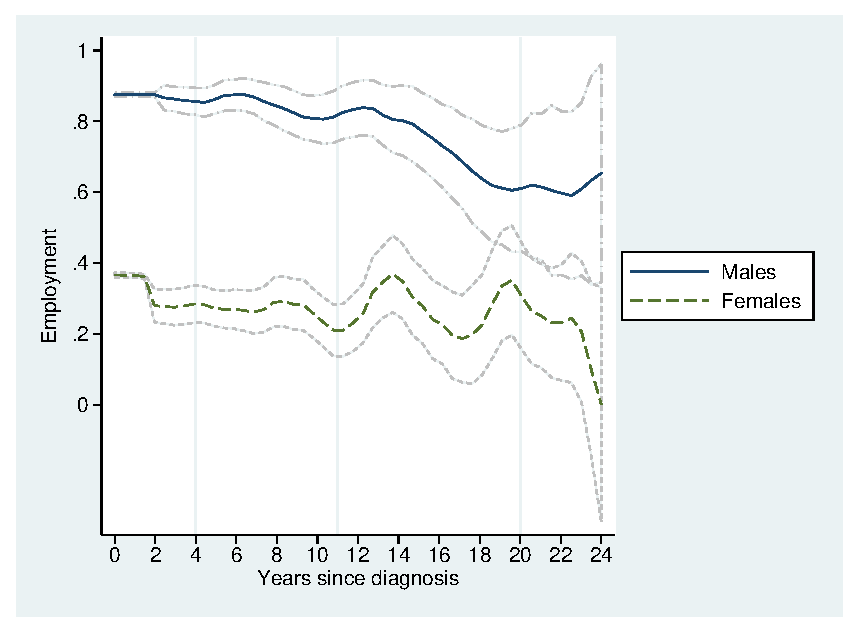
\includegraphics[width=0.8\columnwidth]{Chapter4/Figures/lpoly_works_diabetesduration.eps}\\
\footnotesize{\textit{Notes} The dotted lines around the main line show 95\% confidence intervals.}
\end{center}
\end{figure}
\FloatBarrier
\begin{figure}[h!]
\caption{\label{fig:Kernel-weighted-local-polynomial_wage}Kernel-weighted local
polynomial regression of log hourly wages on diabetes duration.}%
\begin{center}
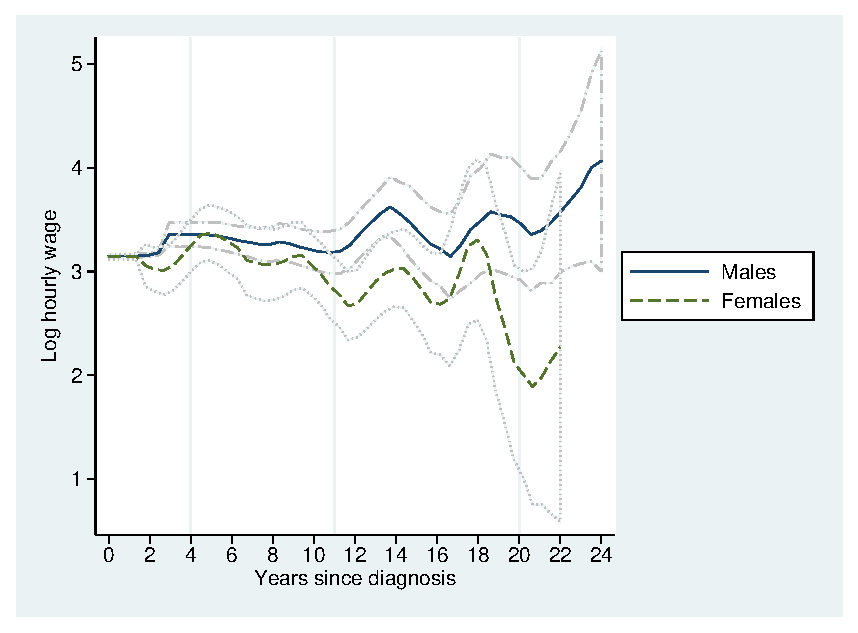
\includegraphics[width=0.8\columnwidth]{Chapter4/Figures/lpoly_wage_diabetesduration.eps}\\
\footnotesize{\textit{Notes} The dotted lines around the main line show 95\% confidence intervals.}
\end{center}
\end{figure}

\begin{figure}[h!]
\caption{\label{fig:Kernel-weighted-local-polynomial_workhrs}Kernel-weighted local
polynomial regression of working hours on diabetes duration.}%
\begin{center}
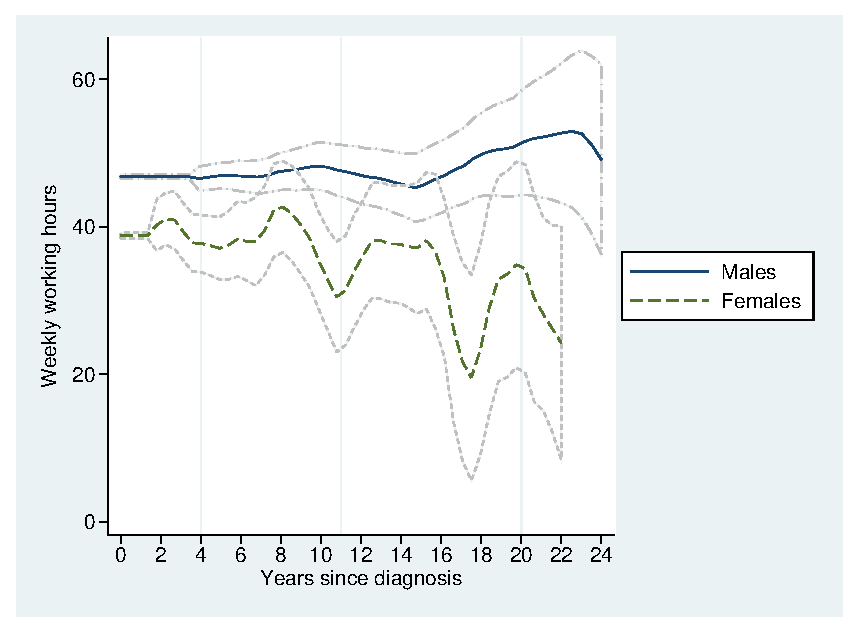
\includegraphics[width=0.8\columnwidth]{Chapter4/Figures/lpoly_workhrs_diabetesduration.eps}\\
\footnotesize{\textit{Notes} The dotted lines around the main line show 95\% confidence intervals.}
\end{center}
\end{figure}
\FloatBarrier

Table \ref{tab:Self-reported-diabetes-duration} presents the results of the linear and non-linear duration models (for which we created the following splines to capture the immediate, intermediate and long-term relationships:0--4,
5--11, 12--19 and 20+), starting with the results of the cross-sectional \ac{LPM}, followed by the pooled \ac{LPM} and then the \ac{FE} model as specified in Eq. (\ref{eq:duration_linear}) and Eq. (\ref{eq:splines}).

For employment probabilities the results indicate a yearly reduction in male employment probability throughout. For women the coefficient shows a reduction of up to almost 1 percentage points per year, though the association is not as strong in the \ac{FE} model. The coefficients in the spline models provide some evidence for an immediate effect of diabetes, which then levels off for some time after which it becomes stronger again. Nonetheless, for males and particularly females, the coefficients are quite imprecisely measured.

\begin{table}
\caption{\label{tab:Self-reported-diabetes-duration}Relationship between self-reported years since diagnosis and labour market outcomes using continuous duration and duration splines.}
\begin{center}
%\resizebox{\linewidth}{!}{%
\begin{adjustbox}{max width=\linewidth}
\begin{threeparttable}

{
\def\sym#1{\ifmmode^{#1}\else\(^{#1}\)\fi}
\begin{tabular}{l*{6}{S
S}}
\toprule
                &\multicolumn{3}{c}{Males}                               &\multicolumn{3}{c}{Females}                             \\\cmidrule(lr){2-4}\cmidrule(lr){5-7}
                &\multicolumn{1}{c}{(1)}&\multicolumn{1}{c}{(2)}&\multicolumn{1}{c}{(3)}&\multicolumn{1}{c}{(4)}&\multicolumn{1}{c}{(5)}&\multicolumn{1}{c}{(6)}\\
                &\multicolumn{1}{c}{OLS (wave 3)}&\multicolumn{1}{c}{Pooled OLS}&\multicolumn{1}{c}{FE}&\multicolumn{1}{c}{OLS (wave 3)}&\multicolumn{1}{c}{Pooled OLS}&\multicolumn{1}{c}{FE}\\
                \addlinespace
\midrule &\multicolumn{6}{c}{\emph{Employment probabilities}} \\ 
\addlinespace
Panel A: &&&&&&\\
Diabetes duration (linear)&   -.008\sym{***}&    -.007\sym{***}&    -.017\sym{***}&    -.005\sym{***}&    -.004\sym{***}&    -.009\sym{*}  \\
                &   (.002)         &   (.002)         &   (.006)         &   (.002)         &   (.001)         &   (.005)         \\
                
\midrule
                Hausman test    &                  &                  &  153.024         &                  &                  &  200.073         \\
                \hspace*{10mm} p-value         &                  &                  &     .000         &                  &                  &     .000         \\
\midrule
\addlinespace
Panel B: &&&&&&\\
Diabetes duration (splines)&&&&&&\\
\hspace*{10mm}0--4&    -.007         &    -.007         &    -.026\sym{*}  &    -.010         &    -.015\sym{**} &    -.017         \\
                &   (.007)         &   (.006)         &   (.014)         &   (.007)         &   (.006)         &   (.016)         \\
\hspace*{10mm}5--11&     .000         &    -.003         &    -.003         &    -.004         &     .004         &    -.003         \\
                &   (.009)         &   (.006)         &   (.009)         &   (.008)         &   (.006)         &   (.008)         \\
\hspace*{10mm}12--20&  -.030\sym{**} &    -.017\sym{*}  &    -.029\sym{*}  &     .005         &    -.004         &    -.014         \\
                &   (.012)         &   (.010)         &   (.016)         &   (.008)         &   (.006)         &   (.011)         \\
\hspace*{10mm}> 20&     .011         &     .007         &    -.046\sym{*}  &    -.010\sym{*}  &    -.003         &    -.015         \\
                &   (.016)         &   (.014)         &   (.028)         &   (.006)         &   (.003)         &   (.018)         \\
\midrule
Hausman test    &                  &                  &  161.953         &                  &                  &  198.692         \\
\hspace*{10mm} p-value         &                  &                  &     .000         &                  &                  &     .000         \\
N               &     8217         &    16292         &    16292         &    10467         &    22407         &    22407         \\
\midrule 
\addlinespace
&\multicolumn{6}{c}{\emph{Log hourly wage}} \\
\addlinespace
Panel A: &&&&&&\\
Diabetes duration (linear)&  .001         &     .010\sym{**} &    -.019         &    -.014\sym{*}  &    -.009         &    -.073\sym{**} \\
                &   (.006)         &   (.005)         &   (.018)         &   (.008)         &   (.008)         &   (.029)         \\
\midrule                
Hausman test    &                  &                  &  838.213         &                  &                  &   93.232         \\
\hspace*{10mm} p-value         &                  &                  &     .000         &                  &                  &     .000         \\                
\midrule
\addlinespace
Panel B: &&&&&&\\
Diabetes duration (splines)&&&&&&\\
\hspace*{10mm}0--4&      .034\sym{*}  &     .046\sym{***}&     .033         &     .027         &     .030         &     .015         \\
                &   (.017)         &   (.016)         &   (.055)         &   (.031)         &   (.026)         &   (.138)         \\
\hspace*{10mm}5--11&    -.041\sym{*}  &    -.037\sym{**} &    -.055\sym{*}  &    -.039         &    -.034         &    -.101\sym{*}  \\
                &   (.021)         &   (.018)         &   (.033)         &   (.030)         &   (.024)         &   (.056)         \\
\hspace*{10mm}12--20&      0.015         &     .044         &     .062         &    -.032         &    -.071\sym{*}  &    -.051         \\
                &   (.033)         &   (.029)         &   (.056)         &   (.042)         &   (.039)         &   (.047)         \\
\hspace*{10mm}> 20&     .053         &     .014         &    -.111         &    -.007         &     .041\sym{***}&    -.204\sym{***}\\
                &   (.054)         &   (.040)         &   (.104)         &   (.028)         &   (.015)         &   (.053)         \\
\midrule
Hausman test    &                  &                  & 1037.290         &                  &                  &   96.266         \\
\hspace*{10mm} p-value         &                  &                  &     .000         &                  &                  &     .000         \\
N               &     5509         &    10767         &    10767         &     2874         &     5741         &     5741         \\
\midrule
\addlinespace
&\multicolumn{6}{c}{\emph{Weekly working hours}}\\
\addlinespace
Panel A: &&&&&&\\
Diabetes duration (linear)& .069         &     .048         &     .181         &    -.020         &    -.124         &     .208         \\
                &   (.124)         &   (.102)         &   (.330)         &   (.187)         &   (.127)         &   (.652)         \\
\midrule
Hausman test    &                  &                  &  704.904         &                  &                  &  107.709         \\
\hspace*{10mm} p-value         &                  &                  &     .000         &                  &                  &     .000         \\
\midrule
\addlinespace
Panel B: &&&&&&\\
Diabetes duration (splines)&&&&&&\\
\hspace*{10mm}0--4&      -.033         &    -.233         &     .709         &     .739         &     .470         &    2.014         \\
                &   (.421)         &   (.325)         &   (.938)         &   (.645)         &   (.586)         &  (2.947)         \\
\hspace*{10mm}5--11&  .269         &     .338         &    -.218         &    -.410         &    -.479         &    -.508         \\
                &   (.539)         &   (.399)         &   (.568)         &   (.728)         &   (.553)         &  (1.020)         \\
\hspace*{10mm}12--20&    .209         &     .137         &     .698         &    -.164         &    -.051         &    -.402         \\
                &   (.730)         &   (.538)         &   (.945)         &   (.995)         &   (.700)         &  (1.207)         \\
\hspace*{10mm}> 20&  -1.300         &    -.768         &     .039         &    -.499         &    -.418         &    8.117\sym{***}\\
                &   (.944)         &   (.930)         &  (2.184)         &   (.930)         &   (.305)         &  (1.612)         \\
\midrule
Hausman test    &                  &                  &  724.225         &                  &                  &  112.627         \\
\hspace*{10mm} p-value         &                  &                  &     .000         &                  &                  &     .000         \\
N               &     6807         &    13581         &    13581         &     3591         &     7383         &     7383         \\
\bottomrule
\end{tabular}
\begin{tablenotes}
\item \textit{Notes} The table presents the results of three estimation methods for the three dependent variables: employment probabilities, log hourly wages and weekly working hours. Panel A presents the results of the linear specifications. Panel B presents the results of the non-linear specifications. Robust standard errors in parentheses. Other control variables: state dummies, urbanization dummies, education dummies, married dummy, number children < 6, wealth, age squared and calendar year dummies. The wage and working hour models additionally control for type of work (agricultural and self employed with dependent non-agricultural wage employment as the base) and for health insurance status. The OLS and pooled OLS models additionally control for age. \sym{*} \(p<0.10\), \sym{**} \(p<0.05\), \sym{***} \(p<0.01\).
\end{tablenotes}
}
\end{threeparttable}
\end{adjustbox}
\end{center}
\end{table}


Turning to wages, the \ac{FE} model indicates a reduction in female wages of about 7\% per year with diabetes. For men we find no consistent effect. The results of the non-linear specification indicate that there may be a reduction in wages 5--11 years after the initial diagnosis. We also find associations for women with more than 20 years of diabetes, but these estimates may be spurious due to the considerably reduced number of observations in this group.\footnote{There are only 9 and 3 observations for male and female wages with more than 20 years since diagnosis in wave 3, respectively, and similarly 17 and 7 in the pooled sample, respectively. For male and female working hours there are 12 and 7 observations with more than 20 years since diagnosis in wave 3, respectively, and 20 and 12 for the pooled sample, respectively.}. There appears to be no consistent relationship between working hours and time since being diagnosed with diabetes.
   

Overall these results suggest a fairly constant decrease in the probability of employment for both men and women and in earnings for women, which contrast with estimates for the USA \parencite{Minor2013}, where no such linear relationship is observed.  \textcite{Minor2013} finds a reduction in employment probabilities of 82 percentage points for females after 11 to 15 years and a reduction of 60 percentage points for males after 2-5 years, indicating very large employment penalties, in particular in comparison to our results for Mexico. However, our non-linear results are not directly comparable to these estimates as Minor used pooled cross-sectional data, constructed dummy variables instead of splines and used different duration groups.\footnote{We estimated a comparable model to that of \textcite{Minor2013} using dummy variables and find a significant reduction in employment chances throughout, regardless of whether we use our duration groups to construct the dummies or the duration groups used by \textcite{Minor2013}. For men, we find a significant reduction of about 6 to 12 percentage points, depending on the used specification, in the first 2 and 4 years after diagnosis, respectively. In the following years the effect size tends to increase somewhat. For women, we find less evidence for an immediate effect of diagnosis, but effects do emerge after about 2 years of living with the disease and also increase somewhat over time. These results are available on request.}
\FloatBarrier

\subsection{Cross-sectional biomarker analysis}


In this section we gain additional insights from using the biomarker data collected in the
third wave of the \ac{MxFLS}. As noted in section \ref{sec:Data}, these data enable us to identify respondents with
\ac{HbA1c} levels equal to or above the internationally recognized diabetes threshold of 6.5\%. This will allow the investigation of the direction of bias introduced when relying on self-reported diabetes only and when it is not possible to identify those unaware as well.

We first present a cross tabulation of self-reported diabetes and the results of the biomarker analysis (Table  \ref{tab:Biomarker_observations}). The table indicates that 27\% of the sample have \ac{HbA1c} levels indicative of diabetes and 81\% of those self-reporting a diabetes diagnosis also have \ac{HbA1c} levels equal to or above the diabetes threshold. Overall, of the people with diabetes according to biomarker analysis, 32\% self-report a diagnosis, while 68\% do not.


\begin{table}[h!]
\caption{\label{tab:Biomarker_observations}Number of observations with diabetes (HbA1c $\geq 6.5\%$) and self-reported diabetes.}
\begin{center}
\begin{adjustbox}{max width=\linewidth}
\begin{threeparttable}
{
\def\sym#1{\ifmmode^{#1}\else\(^{#1}\)\fi}
\begin{tabular}{l*{3}{S S}}
\toprule
            &\multicolumn{1}{c}{$HbA1c < 6.5\%$}&\multicolumn{1}{c}{HbA1c $\geq 6.5\%$}&\multicolumn{1}{c}{Total}\\
\midrule
No self-reported diabetes & 4544 & 1181 & 5725 &  \\
 & 79\% & 21\% & 100\% &  \\
& 97\% & 68\% & 89\% &  \\
Self-reported diabetes & 129 & 554 & 683 &  \\
 & 19\% & 81\% & 100\% &  \\
 & 3\% & 32\% & 11\% &  \\
Total & 4673 & 1735 & 6408 &  \\
 & 73\% & 27\% & 100\% &  \\
  & 100\% & 100\% & 100\% &  \\
\bottomrule
\end{tabular}
\begin{tablenotes}
\item \textit{Notes} The first row of each category presents absolute values, the second row row percentages and the third row column percentages.
\end{tablenotes}
}
\end{threeparttable}
\end{adjustbox}
\end{center}
\end{table}

\FloatBarrier

To further investigate the relationship of self-reported and biomarker tested diabetes, we estimate the models presented in section \ref{sec:Biomarker Strategy}.  
The results in columns 1 and 2 of Table \ref{tab:Biomarker_results} show that the earlier results are robust for the biomarker sample. The coefficients in column 3 and 4 indicate that the associations with employment probabilities are much weaker when using diabetes defined by the biomarker instead of self-reported diabetes.\footnote{We also created a dummy variable that additionally to measured diabetes accounted for those with a self-reported diabetes diagnosis but biomaker levels below the diabetes threshold. This allowed us to investigate the effect for the entire diabetes population. The coefficients and their statistical significance are only marginally different to those presented in columns 3 and 4 of Table \ref{tab:Biomarker_results}, which is why we do not present them here.} In columns 5 and 6, obtained from estimating Eq. \ref{eq:diab_ud}, the coefficient for the biomarker diabetes population $Dbio_i$ now reflects the effect of undiagnosed diabetes, as the regression includes a control for self-reported diabetes, revealing that undiagnosed diabetes is not associated with any of the labour outcomes. The coefficient for self-reported diabetes is marginally bigger in size for men and somewhat smaller for women compared to column 1 and 2, respectively. However, these differences are not statistically significant (p>0.1) using a Z-test, suggesting that not accounting for undiagnosed diabetes will likely leave the estimates of self-reported diabetes unbiased.

\begin{table}[h!]
\caption{\label{tab:Biomarker_results}Biomarker results}
\begin{center}
\begin{adjustbox}{max width=\linewidth}
\begin{threeparttable}
{
\def\sym#1{\ifmmode^{#1}\else\(^{#1}\)\fi}
\begin{tabular}{l*{6}{S
S}}
\toprule
                &\multicolumn{2}{c}{Self-reported diabetes}    &\multicolumn{2}{c}{HbA1c $\geq$ 6.5}&\multicolumn{2}{c}{HbA1c $\geq$ 6.5 and self-reported d.}                 \\\cmidrule(lr){2-3}\cmidrule(lr){4-5}\cmidrule(lr){6-7}
                &\multicolumn{1}{c}{(1)}&\multicolumn{1}{c}{(2)}&\multicolumn{1}{c}{(3)}&\multicolumn{1}{c}{(4)}&\multicolumn{1}{c}{(5)}&\multicolumn{1}{c}{(6)}\\
                &\multicolumn{1}{c}{Males}&\multicolumn{1}{c}{Females}&\multicolumn{1}{c}{Males}&\multicolumn{1}{c}{Females}&\multicolumn{1}{c}{Males}&\multicolumn{1}{c}{Females}\\
\midrule
\multicolumn{7}{l}{\hspace*{10mm}\textbf{Dependent variable: Employment}} \\
Self-reported diabetes&   -.051\sym{**} &    -.044\sym{*}  &                  &                  &    -.053\sym{**} &    -.032         \\
                &   (.026)         &   (.023)         &                  &                  &   (.026)         &   (.026)         \\
HbA1c $\geq$ 6.5&                  &                  &    -.012         &    -.031\sym{*}  &     .003         &    -.022         \\
                &                  &                  &   (.016)         &   (.018)         &   (.017)         &   (.019)         \\
\midrule
N               &\multicolumn{1}{S}{2785}         &\multicolumn{1}{S}{3623}         &\multicolumn{1}{S}{2785}         &\multicolumn{1}{S}{3623}         &\multicolumn{1}{S}{2785}         &\multicolumn{1}{S}{3623}         \\
\midrule
\multicolumn{7}{l}{\hspace*{10mm}\textbf{Dependent variable: Log hourly wages}} \\ 
\addlinespace
Self-reported diabetes&    -.010         &    -.040         &                  &                  &    -.006         &    -.010         \\
                &   (.065)         &   (.113)         &                  &                  &   (.078)         &   (.119)         \\
HbA1c $\geq$ 6.5&                  &                  &    -.007         &    -.057         &    -.006         &    -.055         \\
                &                  &                  &   (.044)         &   (.070)         &   (.049)         &   (.075)         \\
\midrule
N               &\multicolumn{1}{S}{1803}         &\multicolumn{1}{S}{884}         &\multicolumn{1}{S}{1803}         &\multicolumn{1}{S}{884}         &\multicolumn{1}{S}{1803}         &\multicolumn{1}{S}{884}         \\
\midrule
\multicolumn{7}{l}{\hspace*{10mm}\textbf{Dependent variable: Weekly working hours}} \\ 
\addlinespace
Self-reported diabetes&   -.293         &    -.751         &                  &                  &    -.286         &   -1.566         \\
                &  (1.305)         &  (2.178)         &                  &                  &  (1.419)         &  (2.351)         \\
HbA1c $\geq$ 6.5&                  &                  &    -.088         &    1.153         &    -.012         &    1.525         \\
                &                  &                  &   (.844)         &  (1.462)         &   (.925)         &  (1.565)         \\
\bottomrule
\end{tabular}
\begin{tablenotes}
\item \textit{Notes} Community level fixed effects. Robust standard errors in parentheses. Other control variables: age, age squared, state dummies, urbanization dummies, education dummies, married dummy, number children < 6 and wealth. Calender year dummies are included as data collection for the third wave was stretched out over several years. The wage and working hour models additionally control for type of work (agricultural and self employed with non-agricultural wage employment as the base) and for health insurance status. \sym{*} \(p<0.10\), \sym{**} \(p<0.05\), \sym{***} \(p<0.01\).
\end{tablenotes}
}
\end{threeparttable}
\end{adjustbox}
\end{center}
\end{table}

As discussed earlier, differences in effects between self-reported diabetes and those undiagnosed are likely to stem from selection into the diagnosed population, for instance those in worse health or higher \ac{HbA1c} levels are more likely to go to the doctor and be diagnosed as well as to lose their job because of their diabetes. To further explore this, we first estimate models additionally controlling for self-reported health status to capture differences in subjective individual health. Secondly, we investigate in how far differences in measured \ac{HbA1c}, as a proxy for diabetes severity, may explain differences in employment effects of self-reported and undiagnosed diabetes. To this end we estimate Eq. \ref{eq:diab_ud} additionally controlling for \ac{HbA1c} levels.

\begin{table}[h!]
\caption{\label{tab:Diagnosed_undiagnosed_robust}Self-reported diabetes, biomarkers, diabetes severity and self-reported health and their association with labour market outcomes}
\begin{center}
\begin{adjustbox}{max width=\linewidth} 
\begin{threeparttable} 
{
\def\sym#1{\ifmmode^{#1}\else\(^{#1}\)\fi}
\begin{tabular}{l*{6}{S
S}}
\toprule
                &\multicolumn{2}{c}{Employment}       &\multicolumn{2}{c}{Log hourly wages} &\multicolumn{2}{c}{Weekly working hours}\\\cmidrule(lr){2-3}\cmidrule(lr){4-5}\cmidrule(lr){6-7}
                &\multicolumn{1}{c}{(1)}&\multicolumn{1}{c}{(2)}&\multicolumn{1}{c}{(3)}&\multicolumn{1}{c}{(4)}&\multicolumn{1}{c}{(5)}&\multicolumn{1}{c}{(6)}\\
                &\multicolumn{1}{c}{Males}&\multicolumn{1}{c}{Females}&\multicolumn{1}{c}{Males}&\multicolumn{1}{c}{Females}&\multicolumn{1}{c}{Males}&\multicolumn{1}{c}{Females}\\
\midrule
\multicolumn{6}{l}{\hspace*{10mm}\textbf{Panel A (self-reported health)}}\\  
Self-reported diabetes&   -.036         &    -.023         &     .002         &     .060         &     .123         &   -2.191         \\
                &   (.026)         &   (.027)         &   (.079)         &   (.121)         &  (1.433)         &  (2.386)         \\        
Hba1c $\geq 6.5\%$&       .003         &    -.023         &    -.004         &    -.051         &    -.066         &    1.829         \\
                &   (.017)         &   (.019)         &   (.049)         &   (.075)         &   (.926)         &  (1.569)         \\
\multicolumn{6}{l}{Self-reported health status}\\
\hspace*{10mm}good&    .023         &     .057\sym{*}  &     .061         &    -.115         &   -1.131         &    3.521         \\
                &   (.025)         &   (.034)         &   (.074)         &   (.124)         &  (1.376)         &  (2.499)         \\
\hspace*{10mm}fair&    -.007         &     .006         &     .025         &    -.157         &   -1.606         &    4.646\sym{*}  \\
                &   (.026)         &   (.034)         &   (.076)         &   (.128)         &  (1.424)         &  (2.607)         \\
\hspace*{10mm}bad &    -.127\sym{***}&    -.024         &    -.016         &    -.371\sym{*}  &   -6.190\sym{**} &    6.918\sym{*}  \\
                &   (.043)         &   (.046)         &   (.135)         &   (.189)         &  (2.521)         &  (3.858)         \\
\hspace*{10mm}very bad&    -.165         &     .117         &    -.331         &     .316         &   -1.869         &  -17.400\sym{*}  \\
                &   (.110)         &   (.116)         &   (.300)         &   (.439)         &  (6.433)         &  (9.005)         \\
\midrule
N               &\multicolumn{1}{S}{2785}         &\multicolumn{1}{S}{3621}         &\multicolumn{1}{S}{1803}         &\multicolumn{1}{S}{883}         &\multicolumn{1}{S}{2302}         &\multicolumn{1}{S}{1143}         \\
\midrule
\multicolumn{6}{l}{\hspace*{10mm}\textbf{Panel B (HbA1c levels)}}\\
Self-reported diabetes&    -.056\sym{*}  &    -.027         &    -.007         &     .002         &     .076         &   -1.440         \\
                &   (.031)         &   (.025)         &   (.068)         &   (.114)         &  (1.362)         &  (2.382)         \\
\addlinespace
HbA1c $\geq 6.5\%$&    -.005         &    -.005         &    -.010         &    -.019         &    1.032         &    1.887         \\
                &   (.023)         &   (.026)         &   (.060)         &   (.099)         &  (1.279)         &  (2.490)         \\
\addlinespace
HbA1c&     .003         &    -.006         &     .001         &    -.012         &    -.364         &    -.122         \\
                &   (.005)         &   (.006)         &   (.013)         &   (.021)         &   (.279)         &   (.514)         \\
\midrule
N               &     2785         &     3623         &     1803         &      884         &     2302         &     1144         \\
\bottomrule
\end{tabular}
\begin{tablenotes}
\item \textit{Notes} Community level fixed effects. Robust standard errors in parentheses. Other control variables: age, age squared, state dummies, urbanization dummies, education dummies, married dummy, number children < 6 and wealth. Calender year dummies are included as data collection for the third wave was stretched out over several years. The wage and working hour models additionally control for type of work (agricultural and self employed with non-agricultural wage employment as the base) and for health insurance status. \sym{*} \(p<0.10\), \sym{**} \(p<0.05\), \sym{***} \(p<0.01\).
\end{tablenotes}
}
\end{threeparttable}
\end{adjustbox}
\end{center}
\end{table}


When additionally controlling for subjective health status, we find that for men and women the difference between self-reported diabetes and undiagnosed diabetes is reduced due to a smaller coefficient for self-reported diabetes (Table \ref{tab:Diagnosed_undiagnosed_robust}, Panel A). Especially for females, the point estimates for self-reported diabetes and undiagnosed diabetes are now virtually the same size, suggesting that differences can be almost exclusively explained by self-reported health. For men, factors not captured by self-reported health may still play a role. Additionally accounting for measures of overweight and obesity, self-reported hypertension, heart disease and depression does not further affect the interpretation of the diabetes coefficient (results available on request).

Turning to Panel B, we do not find an indication that differences in \ac{HbA1c} levels are driving the different employment effects of diabetes for the aware and unaware. We therefore conclude that current diabetes severity is likely not associated with any labour outcome and does not explain the difference in effects between diagnosed and undiagnosed diabetes.

To the best of our knowledge only one study has previously used biomarkers to analyze the relationship with labour market outcomes in a comparable population. \textcite{BrownIII2011} use data for a Mexican American population in a broadly comparable way to this paper, though stopping short of investigating the labour market impact of undiagnosed diabetes. In concordance with our results this study also finds that once diabetes is diagnosed, current management plays a minor role in determining labour market outcomes. This is not surprising given that \ac{HbA1c} levels only provide a picture of blood glucose levels over the last three months. They therefore may not be representative of blood glucose levels in the years before and after the diabetes diagnosis which ultimately determine how soon complications appear and how severe they will be.
\FloatBarrier


\section{\label{sec:Conclusion}Conclusion}

Diabetes has become one of the most common chronic diseases in middle- and high-income countries, with the potential to severely impact the health and economic well-being of those directly (and possibly indirectly) affected. Yet there remains only limited 'hard' evidence on the economic consequences, especially for these countries. Moreover, what evidence does exist at best partially tackles the econometric challenges involved. 

This paper improves on existing work by addressing several methodological challenges that arise due to the nature of the disease and types of data available, using rich longitudinal panel data from Mexico, a \ac{MIC} for which the biomarker data used in this paper indicates that diabetes, including undiagnosed diabetes, has reached alarming levels.

Apart from providing unique evidence for a developing country, the paper makes methodological contributions for the estimation of labour market effects of diabetes. By estimating individual fixed effects the analysis provides an improved accounting for the endogeneity of self-reported diabetes, as this allows cancelling out the potential role of unobserved individual traits that may affect both labour market outcomes and propensity to self-report (or suffer from) diabetes. Using further information on the year of diagnosis enables us to investigate the potential heterogeneity in the effect of self-reported diabetes on labour market outcomes over time. Finally, taking advantage of biomarker data to identify the entire diabetes population, i.e. including those with undiagnosed diabetes, allows for an assessment of the potential bias in estimates relying on self-reported diabetes (which is still the most frequent measure in the previous literature).

The first part of our results confirms a considerable gap in employment probabilities for both men and women reporting a diabetes diagnosis, compared to those that do not report the condition. Especially women have to deal with a considerable relative reduction in their employment probabilities.  We also find some evidence that diabetes is more likely to reduce the probability of employment in the agricultural and self-employment sector, characterized predominantly by informal arrangements, compared to the rest of the workforce. Those who remain employed do not suffer any wage or labour supply effects, possibly because they are still relatively healthy or are able to resort to a type of work that does not entail their diabetes status limiting their work-related performance. More research will be needed to confirm and further investigate this finding as well as its interpretation. 

Regarding the heterogeneity in the effects of diabetes over time, our results indicate an adverse impact of self-reported diabetes on employment chances, with the impact growing in magnitude especially after the first 10 years post-diagnosis. This is plausible in that as time lived with diabetes evolves, complications associated with diabetes tend to become more frequent and more severe \parencite{Adler2003}. Looking at wages as our labour market outcome, we uncover some adverse effects for females, indicating a sizeable reduction with time since diagnosis. Interestingly, theses reductions in wages appear more or less where no employment effects are found, suggesting that after the initial employment shock fo the diagnosis, reductions in productivity are more levelled, leading only to reductions in wages but not to job loss, at least until further more debilitating complications appear after additional years with the disease.  These findings may bode ill for countries were diabetes has started appearing at an increasingly younger age, causing people to live with the disease for larger parts of their productive lifespan, possibly exacerbating the economic effects of reduced employment due to diabetes \parencite{Hu2011,Villalpando2010}.

The second part of our results indicates that only relying on self-reported diabetes can lead to an overestimation of the relationship between diabetes and labour market outcomes. We find that a negative relationship only exists for those with self-reported, but not for those with undiagnosed diabetes. This perhaps surprising, notable difference, is at least mediated by the subjective health status being worse for those self-reporting compared to the undiagnosed. Current disease severity, as proxied by \ac{HbA1c} levels, does not appear to play an important role in this context.

Our findings bear several implications. First, when interpreting labour market impact estimates relying on self-reported diabetes, one cannot assume that the results extend to those with undiagnosed diabetes. However, the strategy of simply merging self-reported and undiagnosed in one diabetes category may not be ideal, as doing so will fail to account for the heterogeneity between the groups in the amount of health information they possess, the time they have already been exposed to elevated blood glucose levels and consequently their subjective as well as true health status, leading to a potentially important loss of information. If, by contrast, both groups are separately accounted for in the model, thereby acknowledging their inherent differences, this allows us to gain information about the distribution of the economic burden across the two groups. 

Further, the results of the biomarker analysis also reveal that the coefficient of self-reported diabetes is not strongly affected when accounting for biomarker diagnosed diabetes, suggesting that using self-reported diabetes  still provides largely unbiased estimates. The latter estimates should then of course only be used to draw conclusions about the effect of self-reported diabetes, not of diabetes overall. In the case of Mexico, given that more than 7\% of the Mexican population have been diagnosed with diabetes, the identified reduction in employment probabilities still amounts to a significant overall economic burden being associated with (diagnosed) diabetes.

Our results add further weight to the case for reducing the incidence and progression of diabetes. On top of the well-documented health benefits, it appears there are considerable potential gains to be had in terms of increasing the productive lifespan of people. This is of particular importance in \acp{LMIC}, where parental health shocks, related job loss and increasing health expenditures can have repercussions across the entire household. Other family members, including children, may be forced to increase their labour supply and to reduce non-health expenditures in order to prevent deterioration of the household's economic situation. This can lead to forgone investments into child education, showcasing the potential for adverse long-term effects of health shocks due to diabetes \parencite{Bratti2014}. Moreover, the large proportion of undiagnosed people indicates that diagnosis---at least in Mexico---happens too late or not at all, thereby significantly reducing the possibility to prevent complications via appropriate treatment and self-management, which has repercussions by increasing the risk of severe complications appearing early. Hence, much of the health and economic burden may be prevented by earlier diagnosis and, given the generally limited success in achieving good control in Mexico, better treatment of those already diagnosed with diabetes. Ultimately of course, there will be a need to invest in the prevention of diabetes cases in the first place. Taxation of sugar sweetened beverages may be one promising way forward \parencite{Colchero2016}, though the long-term effects in terms of diabetes prevention remain to be demonstrated.





